% Author: Alfredo Sánchez Alberca (asalber@ceu.es)
%----------------------------------------------------------------------------------------
%    DOCUMENT CLASS
%----------------------------------------------------------------------------------------

\documentclass[11pt,a4paper,openright]{book}
%----------------------------------------------------------------------------------------
%	PACKAGES AND OTHER DOCUMENT CONFIGURATIONS
%----------------------------------------------------------------------------------------

% Language settings
\usepackage{polyglossia}
\setdefaultlanguage{english}

% Margins and layout
\usepackage[top=3cm, bottom=3cm, left=2.54cm, right=2.54cm]{geometry}

% Font settings
\usepackage{mathpazo} 
\usepackage{fontspec}
\setmainfont[Ligatures=TeX]{TeX Gyre Pagella}
%\usepackage{unicode-math}
%\setmathfont[math-style=ISO, bold-style=ISO, vargreek-shape=TeX]{TeX Gyre Pagella Math}

% Color
\usepackage{xcolor} % Required for specifying colors by name
\definecolor{color1}{RGB}{5,161,230}
\definecolor{color2}{RGB}{238,50,36}
\definecolor{ocre}{RGB}{243,102,25} % Define the orange color used for highlighting throughout the book
\definecolor{blueceu}{RGB}{5,161,230} % Blue color of CEU logo
\definecolor{greenceu}{RGB}{185,209,16} % Green color of CEU logo
\definecolor{redceu}{RGB}{238,50,36} % Red color of CEU logo
\definecolor{grayceu}{RGB}{111,107,83} % Gray color of CEU logo
\definecolor{coral}{rgb}{1,0.5,0.31} % Orange color for graphics
\definecolor{royalblue1}{rgb}{0.28,0.46,1} % Blue color for graphics
\definecolor{mygreen}{rgb}{0,0.8,0} % Green color for graphics
\definecolor{chaptergrey}{RGB}{5,161,230} % Blue color of CEU logo

% Math support
\usepackage{amsmath} 

% Line breaking
\usepackage{microtype} 
\setlength{\emergencystretch}{2em}

% Graphics
\usepackage{graphicx}
\usepackage{tikz} 
\usepackage{eso-pic} % Required for specifying an image background in the title page

% Arrays and tables
\usepackage{array}
\usepackage{multirow}
\usepackage{colortbl}
\usepackage{booktabs}
\newcommand{\tcrule}{\arrayrulecolor{color1!50!white}\toprule}
\newcommand{\mcrule}{\arrayrulecolor{color1!50!white}\midrule}
\newcommand{\bcrule}{\arrayrulecolor{color1!50!white}\bottomrule}

% Captions
\usepackage[margin=20pt, font=small, labelfont=bf, labelsep=endash]{caption}

% Floating figures
\usepackage{subfigure}

% Lists
\usepackage[shortlabels]{enumitem} % Customize lists
%\setlist{nolistsep} % Reduce spacing between bullet points and numbered lists
\setlist[description]{style=sameline,leftmargin=0cm}

\makeatletter
\let\savees@listquot\es@listquot
\def\es@listquot{\protect\savees@listquot}
\makeatletter

\renewcommand{\theenumiii}{\arabic{enumiii}}

% Flush floating 
\usepackage{afterpage}

% Creative common icons
\usepackage[scale=2]{ccicons}

% hyperlinks
\usepackage{hyperref}
\hypersetup{
pdfauthor = {Alfredo S\'anchez Alberca},
pdftitle = {Calculus with Derive},
pdfsubject = {Calculus},
pdfkeywords = {Maths, Calculus, Derive},
pdfcreator = {XeLaTeX with hyperref package},
pdfproducer = {pdfLaTeX},
colorlinks = true,
linkcolor = red,          % color of internal links
citecolor = green,        % color of links to bibliography
filecolor = magenta,      % color of file links
urlcolor = magenta,          % color of external links
}
%\usepackage{breakurl}

% Indentation
%\setlength\parindent{0pt}

% Control of widow orphan lines
\clubpenalty=10000
\widowpenalty=10000 

%Code listing formatting
\usepackage{listings}
\lstdefinelanguage{morejava}{morekeywords={String}}
\definecolor{vollgrau}{rgb}{0.9,0.9,0.9}
\definecolor{colKeys}{rgb}{0,0,1}
\definecolor{colIdentifier}{rgb}{0,0,0}
\definecolor{colComments}{rgb}{1,0.5,0}
\definecolor{colString}{rgb}{0,0.5,0}
\definecolor{colbackground}{rgb}{0.9,0.9,1}


% Set short or long depending on the version desired
% \usepackage[corto]{optional}

%----------------------------------------------------------------------------------------
%	SECTIONS AND SUBSECTIONS
%----------------------------------------------------------------------------------------
%\titleformat*{\section}{\Huge}
%\titleformat*{\subsection}{\Large}


% Chapter and section formatting 
\usepackage[rigidchapters,explicit]{titlesec}
\setlength{\fboxsep}{5pt}
\newlength{\titulolength}
\setlength{\titulolength}{\textwidth} 
\addtolength{\titulolength}{-2\fboxsep}
\addtolength{\titulolength}{-2\fboxrule}
\titleformat{\chapter}[display]
{\bfseries\sffamily}
{\filleft \mdseries \LARGE \color{blueceu} Practice \Huge\thechapter}
{0.5ex}
{\colorbox{blueceu}{\parbox[t]{\titulolength}{\rule{0mm}{10mm}\Huge\sffamily\filleft\textcolor{white}{#1}}}}
\titleformat{\section}{\normalfont\Large\bfseries\color{blueceu}}{\arabic{section}}{1em}{#1}
\titleformat{\subsection}{\normalfont\large\bfseries\color{blueceu}}{\arabic{section}.\arabic{subsection}}{1em}{#1}
\titleformat{\subsubsection}{\normalfont\normalsize\bfseries\color{blueceu}}{\arabic{section}.\arabic{subsection}.\arabic{subsubsection}}{0.5em}{#1}
\titlespacing{\chapter}{0pt}{0pt}{30ex}
\titlespacing{\section}{0pt}{8ex}{4ex}

%----------------------------------------------------------------------------------------
%	MAIN TABLE OF CONTENTS
%----------------------------------------------------------------------------------------

% \usepackage{titletoc} % Required for manipulating the table of contents
% 
% \contentsmargin{0cm} % Removes the default margin
% % Chapter text styling
% \titlecontents{chapter}[1.25cm] % Indentation
% {\addvspace{15pt}\large\bfseries} % Spacing and font options for chapters
% {\color{gray}\contentslabel[\Large\thecontentslabel.]{1.25cm}} % Chapter number
% {}  
% {\color{gray}\bfseries\hfill\thecontentspage} % Page number
% % Section text styling
% \titlecontents{section}[1.25cm] % Indentation
% {\addvspace{5pt}\bfseries} % Spacing and font options for sections
% {\contentslabel[\thecontentslabel]{1.25cm}} % Section number
% {}
% {\hfill\color{black}\thecontentspage} % Page number
% []
% % Subsection text styling
% \titlecontents{subsection}[1.25cm] % Indentation
% {\addvspace{1pt}\small} % Spacing and font options for subsections
% {\contentslabel[\thecontentslabel]{1.25cm}} % Subsection number
% {}
% {\;\titlerule*[.5pc]{.}\;\thecontentspage} % Page number
% [] 

%----------------------------------------------------------------------------------------
%	MINI TABLE OF CONTENTS IN CHAPTER HEADS
%----------------------------------------------------------------------------------------

% % Section text styling
% \titlecontents{lsection}[0em] % Indendating
% {\footnotesize\sffamily} % Font settings
% {}
% {}
% {}
% 
% % Subsection text styling
% \titlecontents{lsubsection}[.5em] % Indentation
% {\normalfont\footnotesize\sffamily} % Font settings
% {}
% {}
% {}
 
%----------------------------------------------------------------------------------------
%	PAGE HEADERS
%----------------------------------------------------------------------------------------

% Headings and footers
\usepackage{fancyhdr}
\pagestyle{fancy}
\fancyhead{}
\renewcommand{\chaptermark}[1]{\markboth{\thechapter.\ #1}{}}
\fancyhead[LE]{\scshape Calculus with Derive}
\fancyhead[RO]{\sffamily\slshape \leftmark}
\renewcommand{\headrulewidth}{0pt}
\renewcommand{\floatpagefraction}{.8}
\renewcommand{\textfraction}{.1}


% \usepackage{fancyhdr} % Required for header and footer configuration
% 
% \pagestyle{fancy}
% \renewcommand{\chaptermark}[1]{\markboth{\color{grayceu}\sffamily\normalsize\textit{#1}}{}} % Chapter text font
% % settings
% %\renewcommand{\sectionmark}[1]{\markright{\color{grayceu}\sffamily\normalsize\textit{\thesection\hspace{5pt}#1}}{}} %
% % Section text font settings
% \fancyhf{} \fancyfoot[LE,RO]{\normalsize\thepage} % Font setting for the page number in the footer
% \fancyhead[RE]{{\color{grayceu}\sffamily\normalsize\textit{Pr�cticas de Bioestad�stica con R and RKTeaching}}} % Print the nearest
% % section name on the left side of odd pages
% \fancyhead[LO]{\leftmark} % Print the current chapter name on the right side of even pages
% \renewcommand{\headrulewidth}{0pt} % Removes the rule in the header
% \addtolength{\headheight}{2.5pt} % Increase the spacing around the header slightly
% \renewcommand{\footrulewidth}{0pt} % Removes the rule in the footer
% \fancypagestyle{plain}{\fancyhead{}\renewcommand{\headrulewidth}{0pt}} % Style for when a plain pagestyle is specified
% 
% % Removes the header from odd empty pages at the end of chapters
% \makeatletter
% \renewcommand{\cleardoublepage}{
% \clearpage\ifodd\c@page\else
% \hbox{}
% \vspace*{\fill}
% \thispagestyle{empty}
% \newpage
% \fi}


%----------------------------------------------------------------------------------------
%	THEOREM STYLES
%----------------------------------------------------------------------------------------

\usepackage{amsthm} % For including math equations, theorems, symbols, etc

\newcommand{\intoo}[2]{\mathopen{]}#1\,;#2\mathclose{[}}
\newcommand{\ud}{\mathop{\mathrm{{}d}}\mathopen{}}
\newcommand{\intff}[2]{\mathopen{[}#1\,;#2\mathclose{]}}
\newtheorem{notation}{Notation}[chapter]

\newtheoremstyle{blueceu} % Theorem style name
{7pt} % Space above
{7pt} % Space below
{\normalfont} % Body font
{} % Indent amount
{\small\bf\sffamily\color{blueceu}} % Theorem head font
{\;\;} % Punctuation after theorem head
{0.25em} % Space after theorem head
{\small\sffamily\color{blueceu}\thmname{#1}\thmnumber{\@ifnotempty{#1}{ }\@upn{#2}} % Theorem text (e.g. Theorem 2.1)
\thmnote{\ {\the\thm@notefont\sffamily\bfseries\color{blueceu}--- #3.}}} % Optional theorem note
\renewcommand{\qedsymbol}{$\blacksquare$} % Optional qed square

\newtheoremstyle{blacknumex} % Theorem style name
{7pt} % Space above
{7pt} % Space below
{\normalfont} % Body font
{} % Indent amount
{\small\bf\sffamily} % Theorem head font
{\;\;} % Punctuation after theorem head
{0.25em} % Space after theorem head
{\small\sffamily{\tiny\ensuremath{\blacksquare}}\ \thmname{#1}\thmnumber{\@ifnotempty{#1}{ }\@upn{#2}} % Theorem text (e.g. Theorem 2.1)
\thmnote{\ {\the\thm@notefont\sffamily\bfseries--- #3.}}} % Optional theorem note

\newtheoremstyle{blacknum} % Theorem style name
{7pt} % Space above
{7pt} % Space below
{\normalfont} % Body font
{} % Indent amount
{\small\bf\sffamily} % Theorem head font
{\;\;} % Punctuation after theorem head
{0.25em} % Space after theorem head
{\small\sffamily\thmname{#1}\thmnumber{\@ifnotempty{#1}{ }\@upn{#2}} % Theorem text (e.g. Theorem 2.1)
\thmnote{\ {\the\thm@notefont\sffamily\bfseries--- #3.}}} % Optional theorem note

\newtheoremstyle{example} % Theorem style name
{7pt} % Space above
{7pt} % Space below
{\normalfont} % Body font
{} % Indent amount
{\small\bf\sffamily} % Theorem head font
{\;\;} % Punctuation after theorem head
{0.25em} % Space after theorem head
{\small\sffamily\thmname{#1} % Theorem text (e.g. Theorem 2.1)
\thmnote{\ {\the\thm@notefont\sffamily\bfseries--- #3.}}} % Optional theorem note

\newtheoremstyle{indication} % Theorem style name
{-5pt} % Space above
{7pt} % Space below
{\normalfont} % Body font
{-28pt} % Indent amount
{\bf} % Theorem head font
{\kern-11.5pt} % Punctuation after theorem head
{20pt} % Space after theorem head
{\begin{tikzpicture}
\draw node [fill=blueceu,opacity=1,inner sep=1pt] {\makebox[17pt][c]{
\includegraphics[scale=0.3]{img/bulb}}}; \end{tikzpicture}} % Theorem text (e.g. Theorem 2.1)

\makeatother

% Defines the theorem text style for each type of theorem to one of the three styles above
\theoremstyle{ocrenum}
\newtheorem{exerciseT}{Exercise}[chapter]
\theoremstyle{blacknumex}
\newtheorem{exampleT}{Example}[chapter]
%\theoremstyle{blacknum}
\theoremstyle{blueceu}
\newtheorem{vocabulary}{Vocabulary}[chapter]
\newtheorem{definitionT}{Definition}[chapter]
\newtheorem{theoremT}{Theorem}[chapter]
\newtheorem{corolary}{Corolary}[chapter]
\theoremstyle{indication}
\newtheorem{indicationT}{Indication}
%\theoremstyle{example}
%\newtheorem{ejemplo}{Ejemplo}

%----------------------------------------------------------------------------------------
%	DEFINITION OF COLORED BOXES
%----------------------------------------------------------------------------------------

\RequirePackage[framemethod=default]{mdframed} % Required for creating the theorem, definition, exercise and corollary boxes

% Theorem box
\newmdenv[skipabove=7pt,
skipbelow=7pt,
backgroundcolor=black!5,
linecolor=ocre,
innerleftmargin=5pt,
innerrightmargin=5pt,
innertopmargin=5pt,
leftmargin=0cm,
rightmargin=0cm,
innerbottommargin=5pt]{tBox}

% Exercise box	  
\newmdenv[skipabove=7pt,
skipbelow=7pt,
rightline=false,
leftline=true,
topline=false,
bottomline=false,
backgroundcolor=ocre!10,
linecolor=ocre,
innerleftmargin=5pt,
innerrightmargin=5pt,
innertopmargin=5pt,
innerbottommargin=5pt,
leftmargin=0cm,
rightmargin=0cm,
linewidth=4pt]{eBox}	

% Definition box
\newmdenv[skipabove=10pt,
skipbelow=10pt,
rightline=false,
leftline=true,
topline=false,
bottomline=false,
linecolor=ocre,
innerleftmargin=5pt,
innerrightmargin=5pt,
innertopmargin=0pt,
leftmargin=0cm,
rightmargin=0cm,
linewidth=4pt,
innerbottommargin=0pt]{dBox}	

% Corollary box
\newmdenv[skipabove=7pt,
skipbelow=7pt,
rightline=false,
leftline=true,
topline=false,
bottomline=false,
linecolor=gray,
backgroundcolor=black!5,
innerleftmargin=5pt,
innerrightmargin=5pt,
innertopmargin=5pt,
leftmargin=0cm,
rightmargin=0cm,
linewidth=4pt,
innerbottommargin=5pt]{cBox}	

% Indication box
\newmdenv[skipabove=7pt,
skipbelow=7pt,
rightline=false,
leftline=true,
topline=false,
bottomline=false,
linecolor=blueceu,
backgroundcolor=black!5,
innerleftmargin=5pt,
innerrightmargin=5pt,
innertopmargin=5pt,
leftmargin=0pt,
rightmargin=0pt,
linewidth=4pt,
innerbottommargin=5pt]{iBox}		  
		  			  


% Creates an environment for each type of theorem and assigns it a theorem text style from the "Theorem Styles" section above and a colored box from above
\newenvironment{theorem}{\begin{tBox}\begin{theoremT}}{\end{theoremT}\end{tBox}}
\newenvironment{exercise}{\begin{eBox}\begin{exerciseT}}{\hfill{\color{ocre}\tiny\ensuremath{\blacksquare}}\end{exerciseT}\end{eBox}}				  
\newenvironment{definition}{\begin{dBox}\begin{definitionT}}{\end{definitionT}\end{dBox}}	
\newenvironment{example}{\begin{exampleT}}{\hfill{\tiny\ensuremath{\blacksquare}}\end{exampleT}}		
\newenvironment{corollary}{\begin{cBox}\begin{corollaryT}}{\end{corollaryT}\end{cBox}}	
\newenvironment{indication}{\begin{iBox}\begin{indicationT}}{\end{indicationT}\end{iBox}}	

%----------------------------------------------------------------------------------------
%	REMARK ENVIRONMENT
%----------------------------------------------------------------------------------------

%\newenvironment{remark}{\par\vskip10pt\small % Vertical white space above the remark and smaller font size
%\begin{list}{}{
%\leftmargin=35pt % Indentation on the left
%\rightmargin=25pt}\item\ignorespaces % Indentation on the right
%\makebox[-2.5pt]{\begin{tikzpicture}[overlay]
%\node[draw=ocre!60,line width=1pt,circle,fill=ocre!25,font=\sffamily\bfseries,inner sep=2pt,outer sep=0pt] at (-15pt,0pt){\textcolor{ocre}{R}};\end{tikzpicture}} % Orange R in a circle
%\advance\baselineskip -1pt}{\end{list}\vskip5pt} % Tighter line spacing and white space after remark

% %----------------------------------------------------------------------------------------
% %	SECTION NUMBERING IN THE MARGIN
% %----------------------------------------------------------------------------------------
% 
% \makeatletter
% %\renewcommand{\@seccntformat}[1]{\llap{\textcolor{grayceu}{\csname the#1\endcsname.}\hspace{1em}}}                    
% \renewcommand{\section}{
% 	\@startsection{section}{1}{\z@}
% 	{-4ex \@plus -1ex \@minus -.4ex}{1ex \@plus.2ex }
% 	{\normalfont\LARGE}
% }
% \renewcommand{\subsection}{
% 	\@startsection{subsection}{2}{\z@}
% 	{-3ex \@plus -0.1ex \@minus -.4ex}{0.5ex \@plus.2ex }
% 	{\normalfont\Large}
% }
% \renewcommand{\subsubsection}{
% 	\@startsection{subsubsection}{3}{\z@}
% 	{-2ex \@plus -0.1ex \@minus -.2ex}{0.2ex \@plus.2ex }
% 	{\normalfont\large}
% }                        
% \renewcommand{\paragraph}{
% 	\@startsection{paragraph}{4}{\z@}
% 	{-2ex \@plus-.2ex \@minus .2ex}{0.1ex}
% 	{\normalfont\bfseries}
% }
% 
% \def\thechapter{\arabic{chapter}}
% \def\thesection{\thechapter.\arabic{section}.}
% \def\thesubsection{\thesection\arabic{subsection}.}
% \def\thesubsubsection{\thesubsection\arabic{section}.}
% 
% %----------------------------------------------------------------------------------------
% %	CHAPTER HEADINGS
% %----------------------------------------------------------------------------------------
% %\newcommand{\thechapterimage}{}
% %\newcommand{\chapterimage}[1]{\renewcommand{\thechapterimage}{#1}}
% \def\@makechapterhead#1{
% \thispagestyle{empty}
% {
% \ifnum \c@secnumdepth >\m@ne
% \if@mainmatter
% \startcontents
% \begin{tikzpicture}[remember picture,overlay]
% % \node at (current page.north west)
% % {\begin{tikzpicture}[remember picture,overlay]
% % 
% % %\node[anchor=north west] at (-4pt,-27.5mm) {\includegraphics[width=\paperwidth]{\thechapterimage}};
% % %Commenting the 3 lines below removes the small contents box in the chapter heading
% % % \draw[fill=white,opacity=.6] (30mm,-30mm) rectangle (9cm,-9cm);
% % % \node[anchor=north west] at (30mm,-30mm) {\parbox[t][9cm][t]{5.5cm}{\huge\bfseries\flushleft \printcontents{l}{1}{\setcounter{tocdepth}{2}}}};
% % % \draw[anchor=west] (5cm,-11cm) node [rounded corners=25pt,fill=white,opacity=.7,inner sep=15.5pt]{\huge\sffamily\bfseries\textcolor{black}{\vphantom{plPQq}\makebox[20cm]{}}};
% \draw[anchor=north west, fill=black] (0mm,50mm) rectangle (1pt,10mm);
% \draw[anchor=north west] (0cm,20mm) node {\scalebox{1.5}{\Huge{\textcolor{grayceu}\thechapter}}}; 
% %\draw[anchor=west] (0cm,0cm) node {\Huge{#1}}; 
% \end{tikzpicture}
% \par\vspace*{2cm}
% {\Huge #1}
% \par\vspace*{1cm}
% % \end{tikzpicture}}\par\vspace*{230\p@}
% }}
% \def\@makeschapterhead#1{
% \thispagestyle{empty}
% {
% \ifnum \c@secnumdepth >\m@ne
% \if@mainmatter
% \startcontents
% \begin{tikzpicture}[remember picture,overlay]
% % \node at (current page.north west)
% % {\begin{tikzpicture}[remember picture,overlay]
% % \node[anchor=north west] at (-4pt,-27.5mm) {\includegraphics[width=\paperwidth]{\thechapterimage}};
% % \draw[anchor=west] (5cm,-11cm) node [rounded corners=25pt,fill=white,opacity=.7,inner sep=15.5pt]{\huge\sffamily\bfseries\textcolor{black}{\vphantom{plPQq}\makebox[20cm]{}}};
% % \draw[anchor=west] (5cm,-11cm) node [rounded corners=25pt,inner sep=15.5pt]{\huge\sffamily\bfseries\textcolor{black}{#1\vphantom{plPQq}\makebox[20cm]{}}};
% % \end{tikzpicture}};
% % \end{tikzpicture}}\par\vspace*{230\p@}
% %\draw[anchor=west] (0cm,0cm) node {\Huge{#1}}; 
% \end{tikzpicture}
% {\Huge #1}
% \par\vspace*{1cm}
% }}
% \makeatother

 % Insert the commands_book.tex file which contains the majority of the structure behind
% the template

%----------------------------------------------------------------------------------------
%	COMMANDS FOR INDICATIONS
%----------------------------------------------------------------------------------------
\usepackage{menukeys}
\newmenucolortheme{mycolors}{named}{white}{color1}{black}
\changemenucolortheme{menus}{mycolors}
\renewmenumacro{\menu}[>]{menus}
%\newmenustylesimple*{botonstyle}{\textbf{\CurrentMenuElement}}
%\renewmenumacro{\keys}{botonstyle}
\newcommand{\button}[1]{\textsf{\small #1}}
\newcommand{\option}[1]{\textsf{\small #1}}
\newcommand{\mtab}[1]{\textsf{\small #1}}
\newcommand{\field}[1]{\textsf{\small #1}}
\newcommand{\command}[1]{\texttt{#1}}
\newcommand{\variable}[1]{\textsf{\small #1}}
\newcommand{\result}[1]{\texttt{#1}}

% OTHERS
\newcommand{\resetcounters}{\setcounter{page}{1} \setcounter{section}{0} \setcounter{footnote}{0} \setcounter{figure}{0} \setcounter{table}{0}}


%========================================================================================
%   DOCUMENT BODY
%========================================================================================
\begin{document}
\frontmatter 
% Add two blank pages at the begining
%\null\thispagestyle{empty}\newpage
%\null\thispagestyle{empty}\newpage
%----------------------------------------------------------------------------------------
%	TITLE PAGE
%----------------------------------------------------------------------------------------
\begin{titlepage}
\thispagestyle{empty}
\vspace*{7cm}
\par

% Book title
\begin{center}
\normalfont\fontsize{30}{30}\selectfont
{\bfseries \color{blueceu}Calculus with Derive}
\end{center}
\vspace{1cm}

% Authors names
\begin{center}
\Large
\begin{tabular}{c}
%Pablo Ares Gastesi (\url{pablo.aresgastesi@ceu.es})\\
Juan Carlos Garro Garro (\url{garro.eps@ceu.es})\\
Euardo López Ramírez (\url{elopez@ceu.es})\\
José Rojo Montijano (\url{jrojo.eps@ceu.es})\\
Anselmo Romero Limón (\url{arlimon@ceu.es})\\
Alfredo Sánchez Alberca (\href{mailto:asalber@ceu.es}{asalber@ceu.es})\\
Susana Victoria Rodríguez (\url{victoria.eps@ceu.es})
\end{tabular}

\medskip 
Department of Applied Math and Statistics\\ CEU San Pablo\\[1cm]
\medskip 
September 2016

\vspace{1cm}

\includegraphics[height=3cm]{img/logo_uspceu}
\end{center}
\vfill
\end{titlepage} 
%\begin{titlepage}
\AddToShipoutPictureBG*{\includegraphics[width=\paperwidth,height=\paperheight]{img/portada}}
\clearpage
\thispagestyle{empty}
\end{titlepage}

\null\newpage
\thispagestyle{empty}

\null\newpage
\thispagestyle{empty}
%\thispagestyle{empty}
\vspace*{7cm}
\par

% Book title
\begin{center}
\normalfont\fontsize{30}{30}\selectfont
\textsc{\color{blueceu}Bioestadística Aplicada\\ con R and RKTeaching}
\end{center}
\par  
%\vspace*{5mm}
%\hrule
\vspace*{3cm}
% Authors names
\begin{center}
\Large
\begin{tabular}{c}
%Santiago Angulo Díaz-Parreño (\url{sangulo@ceu.es})\\
%Euardo López Ramírez (\url{elopez@ceu.es})\\
%José Rojo Montijano (\url{jrojo.eps@ceu.es})\\
%Anselmo Romero Limón (\url{arlimon@ceu.es})\\
Alfredo Sánchez Alberca\\
\url{asalber@ceu.es}\\
\url{http://aprendeconalf.es}
\end{tabular}
\end{center}

\vspace*{1cm}
\begin{center}
Septiembre de 2014
\end{center}
\par
\vfill
%\includegraphics[scale=0.3]{img/logo_uspceu_01}

\newpage 
 
%----------------------------------------------------------------------------------------
%	COPYRIGHT PAGE
%----------------------------------------------------------------------------------------
\thispagestyle{empty}
\null
\vfill
\hrule depth 3pt
\smallskip
\sffamily

\noindent \textbf{Calculus with Derive}\\
Alfredo Sánchez Alberca (asalber@ceu.es) 

\bigskip
% Creative Commons license terms
{\Large \textbf{License terms \normalsize \ccLogo}}
\medskip

\small
This work is licensed under an Attribution-NonCommercial-ShareAlike 4.0 International Creative Commons License. 
\url{http://creativecommons.org/licenses/by-nc-sa/4.0/}

You are free to: 

\begin{itemize}
\item Share -- copy and redistribute the material in any medium or format
\item Adapt -- remix, transform, and build upon the material
\end{itemize}

Under the following terms:
\begin{center}
\begin{tabular}{cp{0.8\textwidth}}
\ccAttribution &  \textbf{Attribution}. You must give appropriate credit, provide a link
to the license, and indicate if changes were made. You may do so in any reasonable manner, but not in any way that
suggests the licensor endorses you or your use.\\ 
\ccNonCommercialEU & \textbf{NonComercial}. You may not use the material for commercial purposes.\\ 
\ccShareAlike & \textbf{ShareAlike}. If you remix, transform, or build upon the material, you must distribute
your contributions under the same license as the original.
\end{tabular}
\end{center}

No additional restrictions — You may not apply legal terms or technological measures that legally restrict others from
doing anything the license permits.


\normalfont
\newpage

%----------------------------------------------------------------------------------------
%	TABLE OF CONTENTS
%----------------------------------------------------------------------------------------
%\chapterimage{img/chapter_head.png} % Table of contents heading image
{\pagestyle{plain} % No headers
%\input{registro}
\tableofcontents\thispagestyle{empty}
  % Print the table of contents itself
\cleardoublepage % Forces the first chapter to start on an odd page so it's on the right
}

\mainmatter 
%----------------------------------------------------------------------------------------
%	CHAPTERS 
%----------------------------------------------------------------------------------------
% Author: Alfredo Sánchez Alberca (asalber@ceu.es)
\chapter{Introducction to Derive}

\section{Introduction}
In the last decades, the computational power of computers have converted them in powerful tools for disciplines that, as Mathematics, require a large amount of complex computations.

Derive$^{\textsf{\textregistered}}$
\renewcommand{\thefootnote}{\fnsymbol{footnote}}\footnote{These practices are based on version 6.1 of Derive$^{\textregistered}$ for Windows.} is one of the most used programs for doing numerical and symbolic computations.  

Beyond their capabilities for the numerical, vectorial and matrix calculus, it also makes graphical representations. 
This allows to solve a lot of problems of Algebra, Analysis, Calculus, Geometry and even Statistics. 
The advantage of Derive versus other software as Mathematica, Mapple or MATLAB, is its simplicity, what makes it suitable for teaching Maths. 

\begin{center}
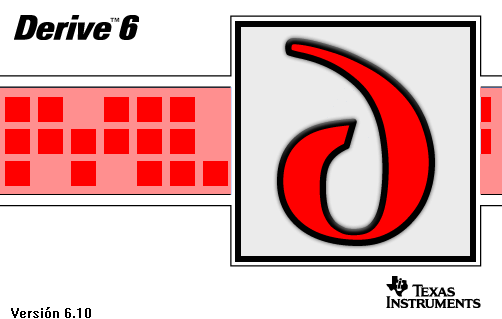
\includegraphics[scale=0.6]{img/introduction/introduction}
\end{center}


The goal of this practice is to introduce the basic usage of this program to the student. 


\section{Basic functionalities}
\subsection*{Starting the program}
As any other Windows applications, to start the program you have to click the \menu{Windows start} button and then select \menu{All the programs > Derive 6} or simply double click the desktop shortcut if there is one. 


\begin{center}
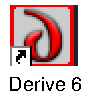
\includegraphics[scale=0.4]{img/introduction/derive_icon}
\end{center}

When the program starts, the main window, that is known as \emph{Algebra window} is shown (figure \ref{g:main}).

\begin{figure}[h!]
\begin{center}
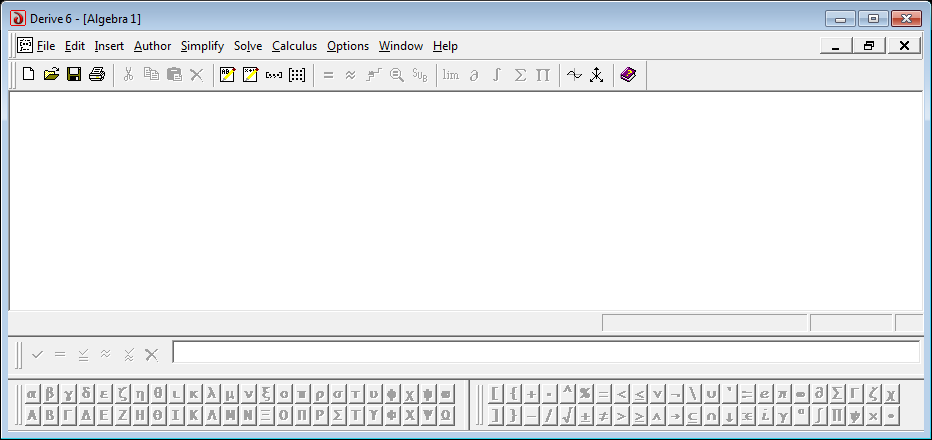
\includegraphics[width=\textwidth]{img/introduction/algebra_window}
\caption{Algebra window of Derive} \label{g:main} 
\end{center}
\end{figure}


The Algebra window has a title bar, a menu bar with menus for all the computations that Derive can performs (limits, derivatives, integrals, graphical representations, etc.), a tool bar with buttons for the main computations, the working area that contains the mathematical expressions that we are working with, the expression editor bar to enter mathematical expressions, the Greek letters and symbols button bar with Greek letters and symbols to enter in expressions and the status bar that shows what is the program doing at any moment. 

\subsection*{Expression edition}
Before doing any computation with a mathematical expression we have to enter it. 

\subsection*{Entering a mathematical expression}
To enter a mathematical expression we use the expression editor bar (figure~\ref{g:expression-editor}), that usually appears at the bottom of the Algebra widows, over the Greeks letters and symbols bar.

\begin{figure}[h!]
\begin{center}

\includegraphics[scale=0.6]{img/introduction/expression_editor}
\caption{Expression editor bar.} \label{g:expression-editor} 
\end{center} 
\end{figure}


In the expression editor bar we can write numbers, letters (that are variables) and symbols and arithmetic and logic operators. 
The most common operators are shown in the table below. 
You can also enter any Greek letter or symbol of the Greek letters and symbols button bar, just clicking on it.


\begin{center}
\begin{tabular}{cc}
\tcrule
\textbf{Symbol} & \textbf{Operator} \\
\texttt{+} & addition \\
\texttt{-} & subtraction \\
\texttt{*} & product \\
\texttt{/} & division \\
\texttt{\^{}} & power \\
\bcrule
\end{tabular}
\end{center}


Operators have different priorities when Derive evaluates a expression. 
First it evaluates functions and constants, second powers, third products and quotients (from left to right) and finally sums and subtractions (from left to right). 
You have to take into account this priority or use parenthesis to force a subexpression to be evaluated before the rest. 
In the following example you have different expressions and what Derive interprets for each of them

\begin{center}\renewcommand{\arraystretch}{2}
\begin{tabular}{cc}
\tcrule
\textbf{Entered expression} & \textbf{Evaluated expression} \\
\texttt{4x-1/x-5} & $4x-\dfrac{1}{x}-5$ \\
\texttt{(4x-1)/x-5} & $\dfrac{4x-1}{x}-5$ \\
\texttt{4x-1/(x-5)} & $4x-\dfrac{1}{x-5}$ \\
\texttt{(4x-1)/(x-5)} & $\dfrac{4x-1}{x-5}$ \\
\bcrule
\end{tabular}
\end{center}

After entering a expression and pressing \button{Enter}, the expression is shown in the working area of the Algebra window, labelled with a tag \verb"#" and a number, such as is shown in the figure~\ref{g:expressions}. 
After that we can reference that expression using its label instead of typing again the expression. 

We can select any expression of the Algebra window click on it. 
If you click several times on the same expression you can select different subexpressions. 
It is also possible to select several consecutive expressions in a block clicking on the first expression and dragging the cursor to the last. 

A useful key is \texttt{F3} that allow entering the selected expression or subexpression in the expression editor bar.

\subsubsection*{Modifying a expression}
Once a expression has been entered, we can modify it clicking on the expression and selecting the menu \menu{Edit > Expression}. 
The expression will be entered in the expression editor bar where you can change whatever you want. 
After making the changes, don't forget to press \button{Enter}. 

\subsubsection*{Removing expressions}
To remove a expression form the working area of the Algebra window, it is enough to select the expression and then press the \button{Supr} key or select the menu \menu{Edit > Delete}.
After removing a expression the labels of the other expressions are renumbered automatically. 
It is also possible to remove blocks of consecutive expressions. 

\textbf{Important!}: If we remove a expression by mistake, it is possible to recover it with the menu \menu{Edit > Undelete}.

\subsubsection*{Rearranging expressions}
It is possible to change the position of any expression in the working area of the Algebra window just clicking on it and, when the expression or block is selected, clicking again on it an dragging it to the new position.  
After arranging a expression the labels of the other expressions are renumbered automatically. 

\subsubsection*{Entering Comments}
The are two ways of entering comments in the working area of the Algebra window. 
The first one is in the expression editor bar, entering the text of the comment in double quotes.
If we proceed this way, the comment will be shown in the working area as any other expression, with its label. 
The second one is with the menu \menu{Insert > Text object}.
If we proceed this other way, the comment will be shown in the working area as an object without label. 

\subsubsection*{Naming variables}
By default Derive uses a single letter to represent variables. 
Thus, the expression \texttt{xy}, is not interpreted as a variable but as the product of variables $x$ and $y$.
Also by default, Derive does not distinguish between lowercase and uppercase letters.
For instance, Derive will interpret the same both if we write \command{cos(x)} or if we write \command{cos(X)}.
Nevertheless, it is possible to configure Derive to use more than one letter for variable names and to be case sensitive with the \menu{Options > Mode settings > Input}.

\subsubsection*{Defining constants and functions}
It is possible to define constants and functions with the operator \command{:=}.
To define a constant it is enough to type the name of the constant followed by \command{:=} and the value of the constant.
For example to define the gravitational constant we can write \command{g:=9.81}. 

To define a function, on the other hand, we have to type the name of the function followed by the list of variables separated by comma in brackets, then \command{:=} and the expression that defines the function. 
Thus, for instance, to define the function that measures the area of a triangle \command{a(b,h):=(b*h)/2} where \command{b} and \command{h} are the variables for the base and the height of the triangle respectively (see figure~\ref{g:expressions}).

With respect to the definition of constants and functions we must be aware of two important facts: 

\begin{itemize}
\item Any time we define a constant or function, the definition is active during all the working session, even if we remove the definition expression.
To remove a definition we have to redefine the constant or function but letting blank the expression after \command{:=}.
For example, to remove the definition of the gravitational constant we have to write \command{g:=}.

\item Derive is case sensitive to function names, so that \command{a(b,h)} and \command{A(b,h)} will be different functions.
\end{itemize}

\subsubsection*{Built-in constants and functions}
Derive has most of the constants and elementary functions used in Mathematics built-in. The syntax of some of them is shown in table ~\ref{t:elementary-functions}.

\begin{table}[h!]
\centering
\begin{tabular}{cl}
\tcrule
\textbf{Syntax} & \textbf{Constant or function} \\
\verb"#"\command{e} & Euler's number $e=2.71828\ldots$ \\
\command{pi} & The number $\pi=3.14159\ldots$ \\
\verb"#"\command{i} & The imaginary number $i=\sqrt{-1}$ \\
\command{inf} & Infinite $\infty$ \\
\command{exp(x)}  & Exponential function $e^x$ \\
\command{log(x,a)} & Logarithmic function with base $a$, $\log_a x$ \\
\command{ln(x)} & Natural logarithmic function $\ln x$ \\
\command{sqrt(x)} & Square root function $\sqrt{x}$ \\
\command{sin(x)} & Sine function $\sin x$ \\
\command{cos(x)} & Cosine function $\cos x$ \\
\command{tan(x)} & Tangent function $\tan x$ \\
\command{asin(x)} & Arcsine function $\arcsin x$ \\
\command{acos(x)} & Arccosine function $\arccos x$ \\
\command{atan(x)} & Arctangent function $\arctan x$ \\
\bcrule
\end{tabular}
\caption{Syntax of some predefined constants and functions.} \label{t:elementary-functions}
\end{table}

In some cases we can also use the symbols of the symbols button bar to refer to these constants.

To know all the built-in constants and functions of Derive we can use the menu \menu{Help > Online} and visit the section \textsf{Built-in Functions and Constants}.

\textbf{Important!}: In built-in functions Derive is not case sensitive.
For instance, the cosine function can be written \command{cos(x)}, \command{Cos(x)} or \command{COS(x)}.

\subsubsection*{Vectors and matrices}
Derive can also deal with vectors and matrices.
To enter a vector you can use the menu \menu{Author > Vector}.
Then enter the number of elements of the vector in the dialog shown and click the \button{OK} button. 
Finally enter the elements of the vector in the dialog shown and click again the \button{OK} button. 
Another way to enter vectors in the expression editor bar is to type their components separated by commas in square brackets. 
For instance, to enter the vector $(x,y,z)$ we write \command{[x,y,z]} (see the figure~\ref{g:expressions}).

To enter matrices we can use the menu \menu{Author > Matrix}.
Then enter the number of rows and columns of the matrix in the dialog shown and click the \button{OK} button. 
Finally enter the elements of the matrix in the dialog shown and click again the \button{OK} button. 

Another way to enter matrices in the expression editor bar is to type their row vectors separated by commas in square brackets. 
For instance, to enter the matrix
\[
\left(
\begin{array}{ccc}
 1 & 2 & 3 \\
 a & b & c \\
\end{array}
\right)
\]
we write \command{[[1,2,3],[a,b,c]]} (see the figure~\ref{g:expressions}).

\begin{figure}[h!]
\begin{center}
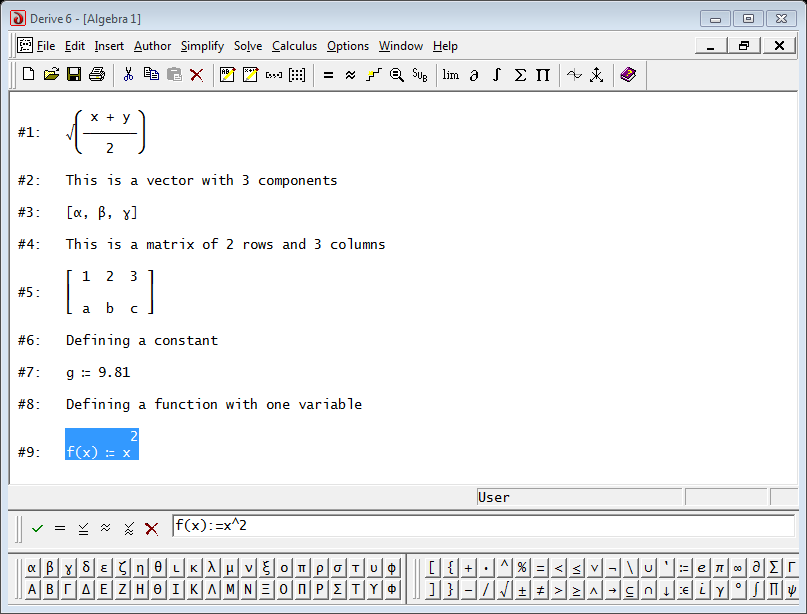
\includegraphics[width=0.8\textwidth]{img/introduction/expressions}
\caption{Different types of expressions in the Algebra window.}
\label{g:expressions}
\end{center}
\end{figure}


\subsection*{Simplifying expressions}
Derive has several ways to simplify expressions.
The simplest one is the basic simplification, that can be done with the menu \menu{Simplify > Basic}. 
This menu performs basic simplifications as, for instance, convert the expression $x+x$ in the expression $2x$. 
However, it doesn't allow to convert the binomial $(x+1)^2$ in $x^2+2x+1$, as it is not clear what of these expressions is simpler. 

To get the expansion of this binomial we can use the menu \menu{Simplify > Expand} that allow to expand a expression with respect to its variables.

On the contrary, if we want to get the binomial from the expanded form, we can use the menu \menu{Simplify > Factor} that allows to factor a expression with respect to its variables.

In any of these simplification types Derive woks in exact mode, what means that decimal numbers are expressed as fractions. 
To get the approximate value of an expression in a decimal form you can use the menu \menu{Simplify > Approximate}. 
This menu shows a dialog where we have to enter the number of decimal places that we want.

Finally, in any expression it is possible to substitute any variable by a value with the menu \menu{Simplify > Variable substitution}.
In the dialog shown you have to select the variable to substitute, enter the value for that variable in the field \field{New value} and click the button \button{OK}.


\subsection*{Graphical representations}
Derive can plot graphical representations in 2 and 3 dimensions.

\subsubsection*{2-dimensional graphical representations}
To represent a function or expression with one variable, we have to select the expression and then the menu \menu{Window > New 2D-plot window}.
This will open a new graphic window with two Cartesian axes ($x$ and $y$).
Finally, to show the graph of the expression in the Cartesian plane you have to select the menu \menu{Insert > Plot} or just click the corresponding button in the toolbar. 
Figure~\ref{g:2d-plot} shows an example of a 2-dimensional plot.

\begin{figure}[h!]
\begin{center}
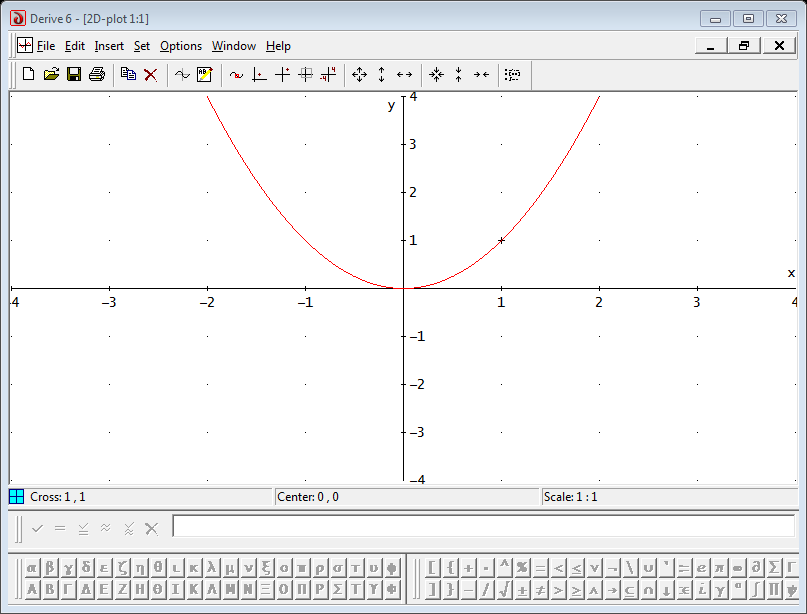
\includegraphics[width=0.8\textwidth]{img/introduction/2d-plot}
\caption{2-dimensional graphic window with the graph of a function.}
\label{g:2d-plot}
\end{center}
\end{figure}

If we want to show the plot in the Algebra window we can use the menu \menu{File > Embed}.

It is possible to represent more than one function in the same 2-dimensional graphic window. 

You can change from the Algebra window to the graphic window and vice versa selecting the corresponding window in the menu \menu{Window}.
However, when you are plotting several expressions is better to see the Algebra and graphic windows at the same time using the \menu{Window > Tile Vertically} (see figure~\ref{g:algebra-2d-plot}.

\begin{figure}[h!]
\begin{center}
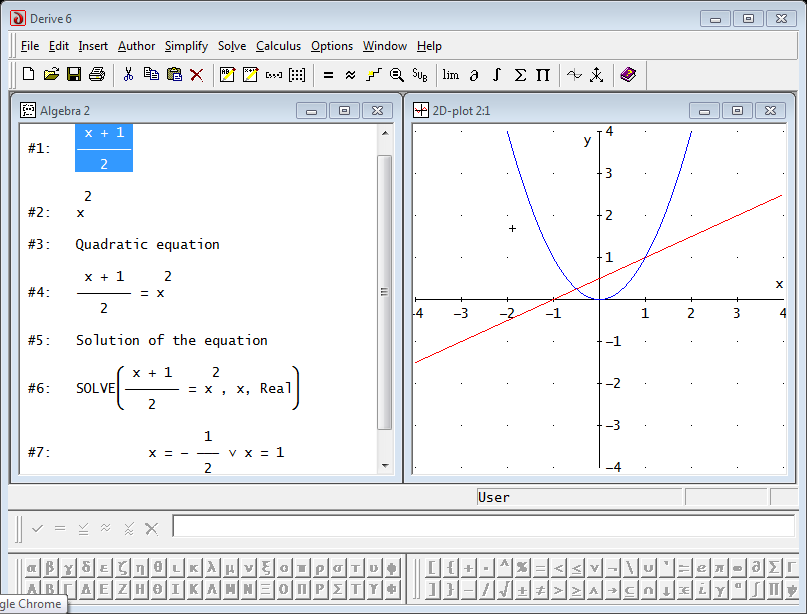
\includegraphics[width=0.8\textwidth]{img/introduction/algebra_2d-plot}
\caption{An Algebra and a 2-dimensional graphic window showed at the same time.} 
\label{g:algebra-2d-plot}
\end{center}
\end{figure}

\subsubsection*{Removing a plot}
To remove the last plot from a graphic window you can use the menu \menu{Edit > Delete plot > Last}. 
It is also possible to remove the first and all the plots but the last with the corresponding menus. 

\subsubsection*{Scaling a plot}
In the graphic window there are several menus and buttons to change the aspect of the plots. 

One of the most interesting actions is changing the scale of axes with the menu \menu{Set > Aspect Ratio}.
It is also possible to change the visible area of the plot with the menu \menu{Set > Plot Range > Minimum/Maximum}. 
In the dialog shown you have to enter the minimum and maximum values for every axis and click the button \button{OK}.


\subsubsection*{Tracing a plot}

In the 2-dimensional graphic windows there is a small cross that we change of position just clicking on a new position of the graphic window.
The coordinates of the cross are always shown in the bottom-left corner of the status bar.
If you press the \command{F3} key, the cross changes to a small square and passes to the \emph{trace mode}.
In this mode the square follows the trajectory of a graph using the arrow keys of the keyboard.
Use the left/right arrows to move the square to the left/right respectively and the up/down arrow to change the graph to follow when there are more than one plot. 
This can be helpful to see the value that takes a function in the graphic window or the points where two graphs intersect (see figure~\ref{g:trace-mode}.

\begin{figure}[h!]
\begin{center}
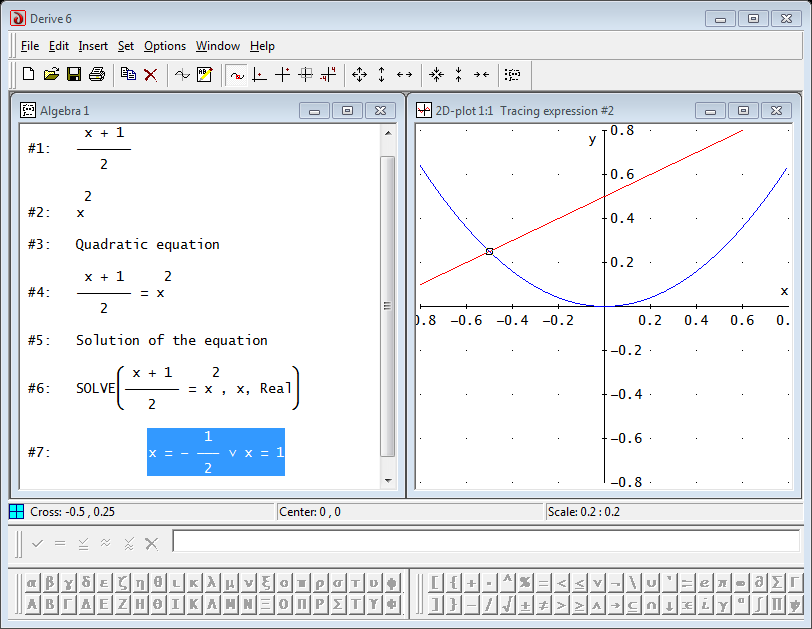
\includegraphics[width=0.8\textwidth]{img/introduction/trace_mode}
\caption{Graphic window in trace mode showing the point where two graphs intersect (that is one solution of the equation).}
\label{g:trace-mode}
\end{center}
\end{figure}


\subsubsection*{Centering the plot}
It is also possible to center the plot at the position of the cross with the button \button{Center on Cross} or at the origin of coordinates with the button \button{Center on Origin}.


\subsubsection*{2-dimensional graphical representations}
To represent a function or expression with 2 variables we have to select the expression and then the menu \menu{Window > New 3D-plot window}.
This will open a new graphic window with three Cartesian axes ($x$, $y$ and $z$).
Finally, to show the graph of the expression in the Cartesian space you have to select the menu \menu{Insert > Plot} or just click the corresponding button in the toolbar. 
Figure~\ref{g:3d-plot} shows an example of a 3-dimensional plot.

\begin{figure}[h!]
\begin{center}
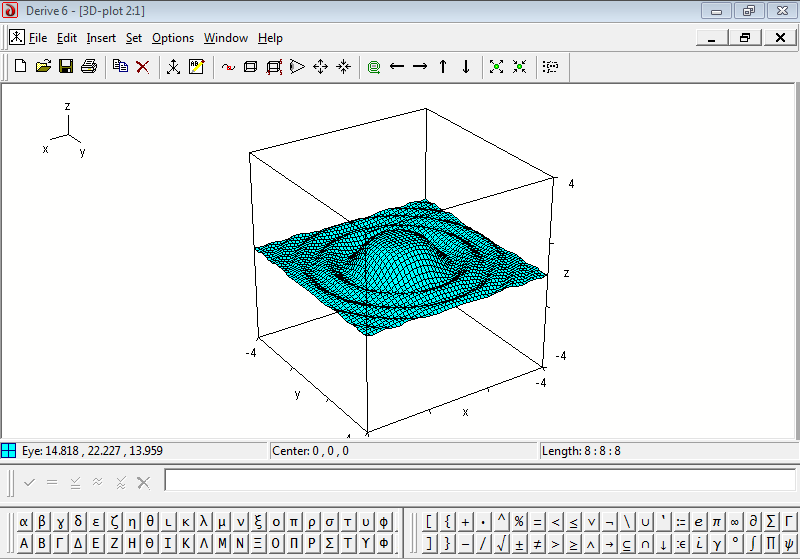
\includegraphics[scale=0.6]{img/introduction/3d-plot}
\caption{3-dimensional graphic window with the graph of a function.}
\label{g:3d-plot}
\end{center}
\end{figure}

Again it is possible to represent more than one function in the same 3-dimensional graphic window. 

Like for 2-dimensional graphic windows, there are several menus an buttons to change the aspect of the plot.

\subsubsection*{Changing the perspective of the plot}
One of the most interesting actions is changing the perspective of the plot with the menu \menu{Set > Eye Position}.
In the dialog shown you have to enter the coordinates of the observer eye and click the button \button{OK}.
It is also possible to change the perspective of the plot rotating the plot horizontally with the left/right arrow keys or vertically with the up/down arrow keys. 

\subsubsection*{Changing the resolution of the grid}
Derive plots the surfaces with a grid of small tiles. 
To change the resolution of the grid you can use the menu \menu{Edit > Plot}. 
In the dialog shown you can enter the number of vertical and horizontal panels.
The higher the number of panels the smoother the surface. 


\subsection*{File management}
The expressions and computations of an Algebra windows can be saved in a file.

\subsubsection*{Saving a file}
To save the content of an Algebra window in a file you can use the menu \menu{File > Save}.
In the dialog shown give a name to the file, select the folder where to save it and click the button \button{Save}.
Derive will put automatically extension \texttt{*.dfw} to the saved file. 
Once the file has been saved, its name will be shown in the title bar of the window. 


\subsubsection*{Opening a file}
To open a Derive file in an Algebra windows you can use the menu \menu{File > Open}.
In the dialog shown you only have to select the file that you want to open an click the button \button{Open}.
The selected file will be opened in a new Algebra window.


\subsubsection*{Opening and closing new Algebra windows}
Derive can manage more than one Algebra windows simultaneously. 
To open a new Algebra window you can use the menu \menu{File > New}. 
Derive works with each Algebra window independently.
That means that we can use the same names to refer to different constants or functions in different Algebra windows without interference. 

On the other side, to close an Algebra window you only have to use the menu 
\menu{File > Close}.


\subsubsection*{Printing}
To print the content of an Algebra window you can use the menu \menu{File > Print}.
However, before printing it is a good idea to preview the document with the menu 
\menu{File > Print Preview}. 
If everything is OK it is enough to click on the button \button{Print} to send the document to the printer. 
To change the margins and the orientation of the page you can use the menu \menu{File > Page Setup}.

Other options like the font, the header or the footer of the page can be set with the menu \menu{Options > Printing > Header and Footer}.


\subsubsection*{Getting help}
Like most Windows applications you can get help about the use of the program with the menu \menu{Help}.

% Author: Alfredo Sánchez Alberca (asalber@ceu.es)
\chapter{Elementary functions}

% \section{Fundamentos teóricos}
% 
% En esta práctica se introducen los conceptos básicos sobre funciones reales de variable real, esto es, funciones
% \[f:\mathbb{R}\rightarrow \mathbb{R}.\]
% 
% \subsection{Dominio e imagen}
% 
% El \emph{Dominio} de la función $f$ es el conjunto de los números
% reales $x$ para los que existe $f(x)$ y se designa mediante $\dom
% f$.
% 
% La \emph{Imagen} de $f$ es el conjunto de los números reales $y$ para los que existe algún $x\in \mathbb{R}$ tal que $f(x)=y$, y se denota por $\im f$.
% 
% 
% \subsection{Signo y crecimiento}
% El \emph{signo} de la función es positivo $(+)$ en los valores de $x$ para los que $f(x)>0$ y negativo $(-)$ en los que $f(x)<0$. Los valores de $x$ en los que la función se anula se conocen como \emph{raíces} de la función.
% 
% Una función $f(x)$ es \emph{creciente} en un intervalo $I$ si $\forall\, x_1, x_2 \in I$ tales que $x_1<x_2$ se verifica que $f(x_1)\leq f(x_2)$.
% 
% Del mismo modo, se dice que una función $f(x)$ es \emph{decreciente} en un intervalo $I$ si $\forall\, x_1, x_2 \in I$ tales que $x_1<x_2$ se verifica que $f(x_1)\geq f(x_2)$. En la figura~\ref{g:crecimiento} se muestran estos conceptos.
% 
% \begin{figure}[h!]
% \centering \subfigure[Función creciente.] {\label{g:funcion_creciente}
% \scalebox{1}{\input{img/funciones_elementales/funcion_creciente}}}\qquad
% \subfigure[Función decreciente.]{\label{g:funcion_decreciente}
% \scalebox{1}{\input{img/funciones_elementales/funcion_decreciente}}}
% \caption{Crecimiento de una función.}
% \label{g:crecimiento}
% \end{figure}
% 
% 
% \subsection{Extremos Relativos}
% Una función $f(x)$ tiene un \emph{máximo relativo} en $x_0$ si existe un entorno $A$ de $x_0$ tal que $\forall x \in A$
% se verifica que $f(x)\leq f(x_0)$.
% 
% Una función $f(x)$ tiene un \emph{mínimo relativo} en $x_0$ si existe un entorno $A$ de $x_0$ tal que $\forall x\in A$
% se verifica que $f(x)\geq f(x_0)$.
% 
% Diremos que la función $f(x)$ tiene un \emph{extremo relativo} en un punto si tiene un \emph{máximo o mínimo relativo}
% en dicho punto. Estos conceptos se muestran en la figura~\ref{g:extremos}.
% 
% \begin{figure}[h!]
% \centering \subfigure[Máximo relativo.] {\label{g:maximo}
% \scalebox{1}{\input{img/funciones_elementales/maximo}}}\qquad
% \subfigure[Mínimo relativo.]{\label{g:minimo}
% \scalebox{1}{\input{img/funciones_elementales/minimo}}}
% \caption{Extremos relativos de una función.}
% \label{g:extremos}
% \end{figure}
% 
% Una función $f(x)$ está \emph{acotada superiormente} si $\exists K\in\mathbb{R}$ tal que $f(x)\leq K$ $\forall x \in \dom f$. Análogamente, se dice que una función $f(x)$ está \emph{acotada inferiormente} si $\exists K\in\mathbb{R}$ tal que $f(x)\geq K$ $\forall x \in \dom f$.
% 
% Una función $f(x)$ está \emph{acotada} si lo está superior e inferiormente, es decir si $\exists K\in\mathbb{R}$ tal que $|f(x)|\leq K$ $\forall x \in \dom f$.
% 
% 
% \subsection{Concavidad}
% 
% De forma intuitiva se puede decir que una función $f(x)$ es \emph{cóncava} en un intervalo $I$ si $\forall\, x_1, x_2
% \in I$, el segmento de extremos $(x_1,f(x_1))$ y $(x_2,f(x_2))$ queda por encima de la gráfica de $f$.
% 
% Análogamente se dirá que es \emph{convexa} si el segmento anterior queda por debajo de la gráfica de $f$.
% 
% Diremos que la función $f(x)$ tiene un \emph{punto de inflexión} en $x_0$ si en ese punto la función pasa de cóncava a
% convexa o de convexa a cóncava. Estos conceptos se ilustran en la figura~\ref{g:concavidad}.
% 
% \begin{figure}[h!]
% \centering \subfigure[Función cóncava.] {\label{g:funcion_concava_arriba}
% \scalebox{1}{\input{img/funciones_elementales/funcion_concava_arriba}}}\qquad
% \subfigure[Función convexa.]{\label{g:funcion_concava_abajo}
% \scalebox{1}{\input{img/funciones_elementales/funcion_concava_abajo}}}
% \caption{Concavidad de una función.}
% \label{g:concavidad}
% \end{figure}
% 
% \subsection{Asíntotas}
% 
% La recta $x=a$ es una \emph{asíntota vertical} de la función $f(x)$ si al menos uno de los límites laterales de $f(x)$ cuando $x$ tiende hacia $a$ es $+\infty$ o $-\infty$, es decir cuando se verifique alguna de las siguientes igualdades
% \[
% \ \lim_{x\rightarrow a^{+}}f(x)=\pm\infty   \quad \textrm{o} \quad
% \lim_{x\rightarrow a^{-}}f(x)=\pm\infty
% \]
% 
% La recta $y=b$ es una \emph{asíntota horizontal} de la función $f(x)$ si alguno de los límites de $f(x)$ cuando $x$ tiende hacia $+\infty$ o $-\infty$ es igual a $b$, es decir cuando se verifique
% \[
% \ \lim_{x\rightarrow -\infty }f(x)=b    \quad \textrm{o} \quad
% \ \lim_{x\rightarrow +\infty }f(x)=b
% \]
% 
% La recta $y=mx+n$ es una \emph{asíntota oblicua} de la función $f(x)$ si alguno de los límites de $f(x)-(mx+n)$ cuando $x$ tiende hacia $+\infty$ o $-\infty$ es igual a 0, es decir si
% 
% \[
% \ \lim_{x\rightarrow -\infty }{(f(x)-mx)}=n    \quad \textrm{o} \quad
% \ \lim_{x\rightarrow +\infty }{(f(x)-mx)}=n
% \]
% 
% En la figura~\ref{g:asintotas} se muestran los distintos tipos de asíntotas.
% 
% \begin{figure}[h!]
% \centering \subfigure[Asíntota horizontal y vertical.] {\label{g:asintotahorizontalyvertical}
% \scalebox{1}{\input{img/funciones_elementales/asintota_vertical_horizontal}}}\qquad\qquad
% \subfigure[Asíntota vertical y oblicua.]{\label{g:asintotaoblicua}
% \scalebox{1}{\input{img/funciones_elementales/asintota_oblicua}}}
% \caption{Tipos de asíntotas de una función.}
% \label{g:asintotas}
% \end{figure}
% 
% 
% \subsection{Periodicidad}
% Una función $f(x)$ es \emph{periódica} si existe $h\in\mathbb{R^{+}}$ tal que \[f(x+h)=f(x)\  \forall x\in \dom f\] siendo el período $T$ de la función, el menor valor $h$ que verifique la igualdad anterior.
% 
% En una función periódica, por ejemplo $f(x)=A\sin(wt)$, se denomina \emph{amplitud} al valor de $A$, y es la mitad de la diferencia entre los valores máximos y mínimos de la función. En la figura~\ref{g:periodoyamplitud} se ilustran estos conceptos.
% 
% \begin{figure}[h!]
% \centering
% \scalebox{0.8}{\input{img/funciones_elementales/funcion_periodica}}
% \caption{Periodo y amplitud de una función periódica.}
% \label{g:periodoyamplitud}
% \end{figure}
% 
% \clearpage
% \newpage

\section{Solved exercises}

\begin{enumerate}[leftmargin=*]
\item Consider the function
\[
f(t)=\frac{t^4+19t^2-5}{t^4+9t^2-10}.
\]
 
\begin{enumerate}
\item Plot the graph of the function. 
\begin{indication}
\begin{enumerate}
\item Enter the expression of the function and select it. 
\item Select the menu \menu{Window > New 2D-plot Window}.
\item In the graphic window click the button \button{Plot}.
\end{enumerate}
\end{indication}

\item Looking at the graph of the function determine:
\begin{enumerate}
\item Domain.
\begin{indication}
Look at the values of $x$ where the function does exists, that is, where there is graph.
\end{indication}

\item  Image.
\begin{indication}
Look at the values of $y$ that are output of the function, that is, where there is graph. 
\end{indication}

\item  Asymptotes.
\begin{indication}
Look at the lines (horizontal, vertical or oblique) where the graph approaches (the distance between the graph and the line tends to zero as they tend to infinity).
\end{indication}

\item  Zeros.
\begin{indication}
Look at the values of $x$  where the graph cuts the horizontal axis. 
\end{indication}

\item Sign.
\begin{indication}
Look at the values of $x$ where the graph is over the horizontal axis (positive) and where it is under the horizontal axis (negative).
\end{indication}

\item Continuity
\begin{indication}
Look at the values of $x$ where you can trace the graph without lifting your hand. 
\end{indication}

\item Increasing and decreasing.
\begin{indication}
Look at the values of $x$ where $y$ increases when $x$ increases (increasing) and the values where $y$ decreases when $x$ increases (decreasing).
\end{indication}

\item Concavity
\begin{indication}
Look at the values of $x$ where the curvature of the graph is up $\cup$ (concave up or convex) and where the curvature is down $\cap$ (concave down or simply concave).
\end{indication}

\item Relative extrema.
\begin{indication}
Look at the values of $x$ where the graph has a peak (relative maximum) and where the graph has a valley (relative minimum).
\end{indication}

\item Inflection points.
\begin{indication}
Look at the values of $x$ where the curvature changes continuously. 
\end{indication}
\end{enumerate}
\end{enumerate}


\item Plot in the same graphic window the graphs of the functions $2^x$, $e^x$, $0.7^x$, $0.5^x$. 
Looking at the graphs of the functions, determine which ones are increasing and which ones are decreasing. 

\begin{indication}
Open a new graphic window with the menu \menu{Window > New 2d-plot Window} and select the menu \menu{Window -> Tile Vertically} to see the Algebra and the graphic windows at the same time. 

For every function repeat the following steps:
\begin{enumerate}
\item Enter the expression of the function in the Algebra window and select it. 
\item Click the button \button{Plot} in the graphic window.
\item Click at some point near the graph and select the menu \menu{Insert > Annotation}. 
In the dialog shown enter the name of the function and click the button \button{OK}.
\end{enumerate}
\end{indication}

Can you deduce for what values of $a$ the function $a^x$ is increasing and for what values it is decreasing?


\item Plot in the same graphic window the graphs of the following functions and determine their periods and amplitudes. 
\begin{enumerate}
\item $\sin(x)$, $\sin(x)+2$, $\sin(x+2)$.
\item $\sin(2x)$, $2\sin(x)$, $\sin(x/2)$.
\begin{indication}
Open a new graphic window with the menu \menu{Window > New 2d-plot Window} and select the menu \menu{Window -> Tile Vertically} to see the Algebra and the graphic windows at the same time. 
For every function repeat the following steps:
\begin{enumerate}
\item Enter the expression of the function in the Algebra window and select it. 
\item Click the button \button{Plot} in the graphic window.
\item Click at some point near the graph and select the menu \menu{Insert > Annotation}. 
In the dialog shown enter the name of the function and click the button \button{OK}.
\end{enumerate}
For the period look at the length of the smaller interval in the horizontal axis where the graph is repeated. 

For the amplitude look at the distance between the maximum and the minimum and divide it by two.
\end{indication}
\end{enumerate}


\item Plot the piecewise function 
\[
f(x)=
\begin{cases}
-2x & \mbox{if $x\leq0$;} \\
x^2 & \mbox{if $x>0$.}
\end{cases}
\]

\begin{indication}
To represent a piecewise function Derive uses the function \command{CHI}.
The syntax for this function is \command{CHI(a,x,b)}, where \command{a} and \command{b} are the lower and upper limits where a subfunction is defined and \command{x} is the variable of the function. 
This defines the function 
\[
\operatorname{CHI} (a,x,b) = 
\begin{cases}
0 & \mbox{if $x<a$} \\
1 & \mbox{if $a\leq x \leq b$} \\
0 & \mbox{if $x>b$}
 \end{cases}
\]

According to this, to enter the piecewise function we have to write  
\[
\command{-2x CHI(-inf,x,0) + x\^{}2 CHI(0,x,inf)}
\]
\end{indication}
\end{enumerate}


\section{Proposed exercises}
\begin{enumerate}[leftmargin=*]
\item Plot the graphs of the following functions and determine their domains looking at their graphs.  

\begin{enumerate}
\item $f(x)=\dfrac{x^2+x+1}{x^3-x}$
\item $g(x)=\sqrt{x^4-1}$.
\item $h(x)=\cos\left(\frac{x+3}{x^2+1}\right)$.
\item $l(x)=\arcsin\left(\frac{x}{1+x}\right)$.
\end{enumerate}

\item Consider the function
\[
f(x)=\frac{x^3+x+2}{5x^3-9x^2-4x+4}.
\]

Plot the function and determine looking at its graph:
\begin{enumerate}
\item Domain
\item Image
\item Asymptotes
\item Zeros
\item Sign
\item Continuity
\item Increasing and decreasing
\item Concavity
\item Relative extrema
\item Inflection points
\end{enumerate}

\item Plot in the same graphic window the graphs of the functions $\log_{10}x$, $\log_{2}x$, $\log x$, $\log_{0.5}x$.
\begin{enumerate}
\item Looking at their graphs determine which funtions are increasing and which ones are decreasing.
\item Deduce for what values of $a$ the function $\log_ax$ is increasing and for what values it is decreasing?
\end{enumerate}

\item Plot the following functions and complete the following sentences with the word equal or the number of times that is lower or greater in any case.
\begin{enumerate}
\item The function $\cos(2x)$ has a period ............ than the function $\cos{x}$.
\item The function $\cos(2x)$ has an amplitude ............ than the function $\cos{x}$.
\item The function $\cos(x/2)$ has period ............ than the function $\cos(3x)$.
\item The function $\cos(x/2)$ has an amplitude ............ than the function $\cos(3x)$.
\item The function $3\cos(2x)$ has a period ............ than the function $\cos(x/2)$.
\item The function $3\cos(2x)$ has an amplitude ............ than the function $\cos(x/2)$.
\end{enumerate}

\item Find the solutions of the equation $e^{-1/x}=\dfrac{1}{x}$  graphically.

\item Plot the graph of the function
\[
f(x)=
\begin{cases}
x^3 & \mbox{if $x<0$} \\
e^x-1 & \mbox{if $x\geq0$}
\end{cases}
\]
\end{enumerate}


% \appendix
\end{document}
